\documentclass[12pt,a4paper]{report}

\usepackage[left=2cm, right=2cm, top=4cm, bottom=2cm]{geometry}
\usepackage{enumitem}
\usepackage{fontspec}
\usepackage{tikz}
\usepackage{amsmath}
\usepackage{algpseudocode}

%Eventos
\algblockdefx[Initially]{Initially}{EndInitially}{\textbf{initially do}}{\textbf{end initially}}
\algblockdefx[Upon]{Upon}{EndUpon}[1]{\textbf{upon #1}}{\textbf{end upon}}

\begin{document}
	%Portada
\begin{titlepage}
	\centering
	{\scshape\LARGE Universidad Nacional Autónoma de México \par}
	\vspace{1cm}
	{\scshape\Large Computación Distribuida\par}
	\vspace{1.5cm}
	{\huge\bfseries Tarea 8\par}
	\vspace{.5cm}
	{\Large\itshape Edgar Quiroz Castañeda \par}
	\vspace{.5cm}
	{\Large\itshape Jerónimo Almeida Rodríguez \par}
	\vfill
	 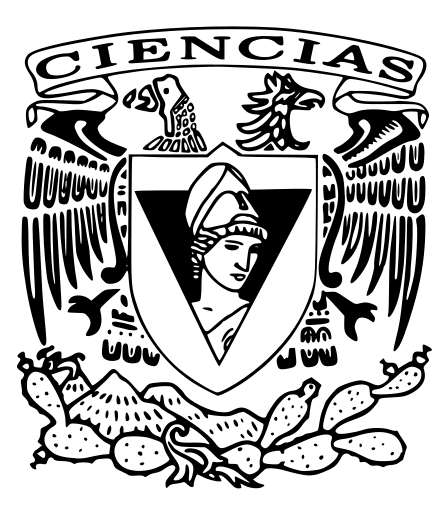
\includegraphics[width=0.5\textwidth]{escudo_f-ciencias.png}
	\vfill

	{\large Jueves 8 de noviembre del 2018 \par}
\end{titlepage}

\pagebreak
\setlength{\voffset}{-0.75in}
\setlength{\headsep}{5pt}

%Ejercicios
\begin{itemize}
\item[1]{Considere el algoritmo 3PC visto en clase. Indique el mínimo y el
    máximo número de rondas posibles en una ejecución del algoritmo (cada
    ronda consiste en una fase de envío de mensajes, ya sea del
    coordinador o de los demas).\\
    La ejecución con el mínimo número de rondas es cuándo el coordinador quiere
    abortar. No envía mensajes a nadie y elige ABORT y los otros procesos eligen
    lo mismo al no recibir mensaje del coordinador. Todo esto sucede en cero
    rondas.\\
    La ejecución en el mayor número de rondas es cuándo todos los procesos
    están de acuerdo en ejecutar. Primero el coordinador envía mensaje a todos
    los procesos pidiendo su voto. Segundo, todos los procesos envían que sí
    quieren ejecutar. Tercero, el coordinador envía un mensaje PRE-COMMIT a
    todos los proceso. Cuarto, todos los procesos envían un ACK al coordinador
    y quinto, el coordinador envía COMMIT y ejecuta. Los otros procesos al
    recibir COMMIT del coordinador ejecutan. Todo esto se hace en cinco rondas.
}
\item[2]{Describa 2 ejecuciones diferentes en las que el algoritmo de 3PC
    falla.\\
    Una ejecución en la que el algoritmo falla es cuándo el coordinador falla
    en la última ronda y envía COMMIT a algunos procesos pero no alcanza a
    enviar COMMIT a todos los procesos. Entonces algunos procesos hacen commit y
    otros abort y la base de datos queda en un estado inconsistente.
    La segunda ejecución en la que falla es cuando un proceso falla antes de
    recibir el commit final. Entonces, ese proceso no se ejecuta aunque los
    otros procesos sí se hayan ejecutado, resultando así en una base de datos
    con estado inconsistente.
}
\item[3]{Explique 5 razones por las cuales es deseable evitar programar con
    timeouts.
    \begin{itemize}
        \item[1]{Estimar los timeouts ideales puede ser complicado.}
        \item[2]{Al estar ligado al reloj físico de la computadora, depende del
            hardware y por lo tanto no es portable.}
        \item[3]{Cómo hay que mantener un timeout para cada pareja de procesos,
            no es escalable.}
        \item[4]{Son difíciles de programar.}
        \item[5]{En una red, la variabilidad de los retardos puede ser muy
            grande y por lo tanto difícil de acotar.}
        \item[6]{Cómo los retardos crecen arbitrariamente, pueden ser muy
            grandes, haciendo el sistema muy propenso a errores.}
    \end{itemize}
}
\item[4]{Explique de manera intuitiva la demostracion de correctez del
    algoritmo de Consenso basado en S mostrado en la figura dada.
}
\item[5]{Presente una ejecucion con $t=\tfrac{n}{2}$ en la que el algoritmo
    de la figura dada falla.\\
    Digamos que en una ronda $i$ fallan los $\tfrac{n}{2}$ procesos. Entonces
    los demás procesos se quedarían esperando en la línea $(8)$ pero solo pueden
    recibir $\tfrac{n}{2}-1$ mensajes que es menos de la mayoría. Entonces, el
    algoritmo no acaba.
}
\item[6]{Lea los siguientes 5 sueños de Einstein del libro.
    \begin{itemize}[label=$\bullet$]
        \item{\textbf{28 April 1905}\\
            En este mundo, hay una constante: el tiempo. El tiempo es algo
            inmutable que existe y se mueve igual en cualquier esquina del
            universo. En la tierra, en todos lados se puede ver el tiempo; en
            torres, paredes, incluso la gente carga sus propios medidores del
            tiempo (relojes). Cada día, la gente detiene sus actividades por
            unos instantes para adorar la perfección del tiempo y sincronizar
            sus relojes.\\
            Los religiosos incluso argumentan que la misma perfección del tiempo
            es prueba de existencia de lo divino.\\
            Lo que es cierto es que la gente se refugia en su perfección, pues
            en un mundo en el que las cosas pueden salir mal o de manera
            inesperada, la gente sabe que se puede refugiar en la perfección del
            tiempo, que es universal para todos.
        }
        \item{\textbf{3 May 1905}\\
            En este sueño no existe una relación causal entre causa y efecto. No
            hay manera de determinar si un evento sucedió cómo resultado del
            otro o si es la causa.\\
            Por ejemplo, un país prohibe las armas de fuego y un mes después se
            desata una de las peores olas de crímen en la historia. ¿Esto
            último es el resultado de lo primero o una causa colocada de una
            manera distinta a la que estamos acostumbrados?\\
            Los científicos no tienen prestigio, pues sus predicciónes se han
            vuelto descripciones. \\
            En este mundo, la gente vive sin temer por las consecuencias que sus
            acciones puedan traer en el futuro, pues esas consecuencias ya
            sucedieron.
        }
        \item{\textbf{4 May 1905}\\
            En este mundo el tiempo transcurre pero no sucede mucho. Esto sucede
            para cualquier métrica: de una hora a otra transcurre tan poco cómo
            de un día a otro, de un més a otro e incluso de un año a otro. El
            tiempo pasa pero no hay un cambio sustancial. Un niño de un año a
            otro solamente tiene un año más. Esta es la forma en la que se mueve
            el tiempo en este mundo.
        }
        \item{\textbf{8 May 1905}\\
            El mundo va a acabar el 26 de septiembre de 1907. Todos lo saben.\\
            A medida que esta fecha se va acercando se puede ver cómo las
            actividades van cambiando. Los niños dejan de ir a clases, pues qué
            caso tiene prepararlos para el futuro si no va a haber un futuro.
            Luego, la gente comienza a dejar de ir a trabajar. ¿Para qué
            trabajar para alguién más si de todas maneras todo va a terminar?\\
            A la gente le deja de importar el dinero y empieza a apreciar el
            tiempo que queda. Ya no corre sino que disfruta cada momento.
            Vecinos que nunca se hablaron, ahora conversan cómo mejores amigos
            padres e hijos intentan recuperar aquella relación que dejaron que
            el tiempo marchitara, etc.\\
            En los últimos momentos, la humanidad se une para recibir el fin
            cómo uno.
        }
        \item{\textbf{10 May 1905}\\
            Hay varias maneras de describir el tiempo. En este sueño, el tiempo
            es pegajoso. Uno puede ir a una ciudad y ver vestigios de diferentes
            épocas, incluyendo la actual. Lo sorprendente no es ver los
            vestigios, sino que hay gente que aún habita en ellos. Las personas
            se quedan atrapadas en un momento de sus vidas, del cual no pueden
            escapar. El mundo alrededor sigue, pero la gente no lo percibe. El
            problema de este mundo es que se vive en soledad, pues el pasado no
            puede convivir con el presente y por lo tanto una persona que se ha
            atascado en una época no puede escapar y no hay con quen comparta
            esa época.
        }
    \end{itemize}
}
\end{itemize}
\end{document}
